\documentclass[authoryear,letterpaper,english,12pt]{elsarticle}


\begin{frontmatter}




    \title{American Disclosure Options}
    
    \begin{aug}
    
    \author[id=au1,addressref={add1}]{\fnms{Kerry}~\snm{Back}\ead[label=e1]{kerry.e.back@rice.edu}}
    \author[id=au2,addressref={add2}]{\fnms{Bruce I.}~\snm{Carlin}\ead[label=e2]{bruce.carlin@rice.edu}}
    \author[id=au3,addressref={add2}]{\fnms{Seyed Mohammad}~\snm{Kazempour}\ead[label=e3]{smkazempour@rice.edu}}
    \author[id=au4,addressref={add3}]{\fnms{Chloe L.}~\snm{Xie}\ead[label=e4]{chloexie@mit.edu}}
    
    \address[id=add1]{%
    \orgdiv{Jones Graduate School of Business and School of Social Sciences},
    \orgname{Rice University}}
    
    \address[id=add2]{%
    \orgdiv{Jones Graduate School of Business},
    \orgname{Rice University}}
    
    \address[id=add3]{%
    \orgdiv{Sloan School of Management},
    \orgname{M.I.T.}}
    
    \end{aug}
    
    
    \begin{abstract}
    Abstract goes here.
    \end{abstract}
    
    
    
    \end{frontmatter}
    


\begin{document}



\newpage

\section{Introduction}\label{s:intro}

We study firms with correlated values who have private signals and discretion over when to disclose their signals to the market.  We assume firms wish to maximize their intertemporal average stock prices. Each firm's option to disclose is an American exchange option.  Prior to exercise, each firm is priced by risk-averse investors according to the investors' perception of the firm's value.  The assumption that firms care about average prices means that the price is a ``dividend stream'' received by the firm.  If the firm exercises its exchange option (discloses its signal), then it gives up this dividend stream in exchange for a different dividend stream, namely its price as determined by its private signal.  The value of the asset with which the firm is endowed (its pre-disclosure price) varies stochastically depending on the disclosures of other firms, so each firm's optimal time to exercise depends on the disclosure policies of other firms, each of which in equilibrium also depends on the disclosure policies of others.

This is a particular type of option game.  To our knowledge, this game has not previously been studied.  The static game under risk neutrality dates to Grossman, Milgrom, Dye.  Risk aversion in the static game was introduced by Dye and Hughes but only with a single firm.  Dynamic disclosure is studied by ADK but also with only a single firm and with risk neutrality.  So, our multiple firm model is new both because it includes risk aversion and because it is dynamic.

Equilibrium policies are threshold policies with stochastic thresholds, meaning that at each point in time there is a minimum signal value (threshold), depending on prior disclosures or nondisclosures by other firms, such that it is optimal to disclose if and only if one's signal is above the threshold.  Conditional on a disclosure, there is a nonzero probability that the disclosing firm's signal is exactly equal to the threshold, which we call a ``minimum disclosure.''  It turns out that a key issue in the analysis of the game is whether minimum disclosures make other firms more or less likely to disclose.  This is essentially a question of whether minimum disclosures are good or bad news.  Good news causes prices to rise and makes other firms less likely to disclose; bad news causes prices to fall and make other firms more likely to disclose.\footnote{ADK derive this clustering effect of bad news for exogenous news.}  We show that in the case of two firms, a minimum disclosure is bad news and makes the other firm more likely to disclose.  Based on this result, we characterize the equilibrium fully for the case of two firms.  We conjecture that this result about minimum disclosures applies also for more than two firms.  Conditional on the conjecture, we are able to fully characterize the equilibrium for an arbitrary number of firms.



\section{Model}\label{s:model}




We analyze information disclosure by $n$ firms on a time interval $[0,1]$.  There is a representative investor with constant absolute risk aversion.
Firms learn their date--1 values $\tilde x_i$ at independent uniformly distributed times $\tilde \theta_i \in [0,1]$.  The values are symmetrically and joint normally distributed with the representative investor's date--1 wealth $\tilde w$, which implies that there are constants $\alpha$ and $\beta$ such that, for each $i$,
\begin{equation}
  \tilde x_i =  \alpha + \beta  \tilde w + \tilde \varepsilon_i
\end{equation} 
where the $\tilde \varepsilon_i$ are normally distributed mean-zero variables that are independent of $ \tilde w$.  Assume the $\tilde \varepsilon_i$ are also independent of each other (the single-index model).   Denote the mean and standard deviation of $\tilde w$ by $\mu_w$ and $\sigma_w$, respectively.
Let $\mu= \alpha + \beta \mu_w$ denote the mean of $\tilde x_i$, and let  $\sigma_\varepsilon$ denote the standard deviation of $\tilde \varepsilon_i$.  The variance of $\tilde x_i$ is $\sigma^2 =  \beta^2\sigma_w^2 + \sigma_\varepsilon^2$.  
The correlation of $\tilde x_i$ with $\tilde x_j$ is $\rho = \beta^2\sigma_w^2/\sigma^2$.

Assume the interest rate $r$ is constant.  For convenience, we normalize it to zero.
The stochastic discount factor (SDF) at date 0 for pricing payoffs at date~1 is proportional to the representative investor's marginal utility, which is proportional to  $\E^{-\gamma \tilde w}$.  Because the interest rate is zero, the SDF is 
\begin{equation}
 \tilde m \ = \ \frac{\E^{-\gamma \tilde w}}{\mye[\E^{-\gamma \tilde w}]}\,.
\end{equation}
  We will use risk-neutral pricing.  The risk-neutral expectation of any random variable $\tilde y$ is $\mye^*[\tilde y] = \mye[\tilde m\tilde x]$.
  Assume the information arrival times $\tilde \theta_i$ are independent of $\tilde w$ and hence independent of $\tilde m$.
  
  Lemma~\ref{lemma:riskneutral} states that  the risk-neutral and physical distributions differ only with regard to means, which is a standard result in this CARA/normal setting. The risk premium $\gamma\beta\sigma_w^2$ in Lemma~\ref{lemma:riskneutral} equals risk aversion multiplied by the covariance of the firm value $\tilde x_i$ with the representative investor's wealth~$\tilde w$, as in the CAPM.  The CAPM holds in our model at date~0 but not at subsequent dates, due to the non-normalities induced by investors' inferences.

\begin{lemma}\label{lemma:riskneutral}
Under the risk-neutral probability, the following are true.  The firm values $\tilde x_i$ are joint normally distributed with means $\mu^*  = \mu  - \alpha b\sigma^2$ and with the same standard deviations and correlation as under the physical probability.  Furthermore, they are independent of the information arrival times $\theta_i$, which are independent and uniformly distributed, as under the physical probability.
\end{lemma}  

Assume no information arrives to the market between $0$ and $1$ other than through the disclosures of firms (or the absence of disclosures).  Let $P_t$ denote the price at date $t$ of all firms that have not disclosed (the pool price).  This price evolves deterministically between disclosures and jumps up or down when there is a disclosure.  After a firm discloses, its price is $\tilde x_i$.  

Assume the firm's objective is to choose a disclosure date $\tau \ge \tilde \theta_i$ to maximize
\begin{equation}\label{objective}
 \mye^* \left[\int_0^\tau P_t \,\D t \mid \tilde x_i \right]  + (1-\tau)\tilde x_i \,.
\end{equation}
For any time $t$ prior to $\tilde \theta_i$, the firm has no choice but to remain silent. However, for $t \geq \tilde \theta_i$, it optimally chooses $\tau$ to maximize its price from $t$ onward. The disclosure date $\tau$ is chosen based on all information prior to that date, including the firm's own value and any disclosures made by other firms. Our choice of the objective function \eqref{objective} is motivated by the assumption that the firm or its managers benefit from having a higher share price over the course of time until date~1. For simplicity, we assume the benefit is additive in time and that the benefit is valued according to the market's SDF, producing the objective \eqref{objective}.

We need to work with the conditional distributions that arise as firms disclose their values.  It is convenient to define these inductively.  Put subscripts $n$ on the unconditional parameters $\mu$, $\mu^*$, $\sigma$, and $\rho$.  This indicates that there are $n$ firms that have not yet disclosed.  Order the firms in the reverse order of disclosure, so firm $n$ is the firm that discloses first, etc.  For any $1< k \le n$, define
\begin{subequations}\label{parameter_recursion}
\begin{align}
\mu_{k-1}(\tilde x_k, \ldots \tilde x_n) \ & = \ \rho_{k} \tilde x_{k} + (1-\rho_{k})\mu_{k}(\tilde x_{k+1},\ldots \tilde x_{N})\\
\mu^*_{k-1}(\tilde x_k, \ldots \tilde x_Nn) \ & = \ \rho_{k} \tilde x_k + (1-\rho_{k})\mu^*_{k}(\tilde x_{k+1}, \ldots \tilde x_{n})\\
\sigma_{k-1} \ & = \ \sigma_{k}\sqrt{1-\rho_{k}^2}\\
\rho_{k-1} \ & = \ \frac{\rho_{k}}{1+\rho_{k}}\,. \label{rhon}
\end{align}
\end{subequations}

\begin{lemma}
Conditional on $\tilde x_{k+1}, \ldots, \tilde x_n$, the random variables $\tilde x_{1}, \ldots, \tilde x_k$ are joint normal under the physical probability with means $\mu_k(\tilde x_{k+1}, \ldots \tilde x_n)$, standard deviations $\sigma_k$ and correlation $\rho_k$.  The distribution is the same under the risk-neutral probability except that the means are $\mu^*_{k}(\tilde x_{k+1}, \ldots \tilde x_n)$.
\end{lemma}

\section{Equilibrium}

We consider `threshold strategies,' meaning that at each date $t$, there is a random variable $B_t$, depending on information at $t$, such that each firm $i$ that has received its signal and has not disclosed at $t$ will disclose at $t$ if and only if $\tilde x_i \ge B_t$.  This is equivalent to assuming that if a firm with signal $x$ chooses to disclose at $t$, then all firms with signals $y>x$ will also  disclose.  There is greater urgency for firms with high values to disclose, because they lose more by trading at prices below their values, so the assumption that higher types disclose first is very natural.

We assume that the threshold or boundary $B_t$ is a continuous decreasing function of time between disclosure dates.  The assumption that it is decreasing is motivated by the fact that the price will be decreasing between disclosure dates, because as time passes it becomes more likely that firms have received their signals, and nondisclosure then indicates that the signals are low.  The boundary can jump up or down when a firm discloses, depending on the content of the disclosure.

%%%%%%%%%%%%%%%%%%%%%%%%%%%%%%%%%%%%%%%%%%%%%%%%%%%%%%%%%%
%
\subsection{Equilibrium Price}
%
%%%%%%%%%%%%%%%%%%%%%%%%%%%%%%%%%%%%%%%%%%%%%%%%%%%%%%%%%%

We can express the price in terms of the history of the boundary.  For each date $t$ and each $s<t$, define
$$C_{st} \ = \  \min_{s\le u \le t} B_u\,.$$
This is the `forward looking' minimum of the boundary at date $s$, looking forward through~$t$.  It matters for pricing because the market knows at $t$ that some firm(s) may have received its signal before $t$ -- say, at $s<t$ -- and has not yet disclosed because its signal was below the threshold at all dates between $s$ and $t$.  This means that its signal is below $C_{st}$.  Because the market does not know the date $s$ at which the firm received its signal (or even if it has received a signal at all) it has to integrate over $s$.  As a result of these calculations, the equilibrium price is as follows.  Let $\phi$ and $\Phi$ denote the standard normal density and distribution function respectively.  The integrals in \eqref{price} below are actually finite sums, because $C_{st}$ is a step function in $s$.  The number, timing, and sizes of steps depend on the history of disclosures.  

\begin{proposition}\label{prop:price}
At any date $t$, let $k$ denote the number of firms that have not yet disclosed and denote the disclosures of the other firms by $x_{k+1},\ldots, x_n$.  
The price of the firms that have not disclosed is
\begin{equation}\label{price}
P_t \ = \  \left[\mu^*_k - \sigma_k\frac{\int_0^t \phi\left(\frac{\mu^*_k-C_{st}}{\sigma_k}\right)\,\D s}{1 - \int_0^t \Phi\left(\frac{\mu^*_k-C_{st}}{\sigma_k}\right)\,\D s}\right]\,,
\end{equation}
where we use $\mu^*_k$ as shorthand for $\mu^*_k(x_{k+1},\ldots, x_n)$.  
\end{proposition} 

\subsection{The Disclosure Option}\label{ss:option}

When multiple firms have correlated values and some have not yet disclosed, it may be optimal for a firm to continue to exercise plausible deniability even after the pool price drops below its value. This is due to the possibility that another firm may become informed, disclose a high value, and cause the pool price to jump upwards, which prolongs the value of plausible deniability.  In other words, like typical American options, the disclosure option must be sufficiently far in the money before it is optimal to exercise it.\footnote{\citet*{adk} describe this same real option effect relative to the exogenous announcement that they study.  The difference in our model is that all announcements are endogenous.  Each firm takes into account the option values created by others, and, in turn, each firm's optimal reaction to the option value affects the options values of all other correlated firms.}

We analyze this disclosure option like any other American option. The optimal disclosure threshold is determined by a differential equation in the inaction region, in conjunction with value matching and smooth pasting conditions at the boundary of the region.     At each date~$t$ after a firm learns its value $\tilde x_i$, define the value function
\begin{equation}\label{Jt}
J_t \ = \  \sup_\tau \; \mye^*_t \left[\int_t^\tau P_u \,\D u \mid \tilde x_i \right] + (1-\tau)\tilde x_i\\,.
\end{equation}
The supremum in \eqref{Jt} is taken over disclosure times that can depend on all prior information, and the value \eqref{Jt} depends on all prior disclosures and on the firm's value $\tilde x_i$.  

We can rewrite \eqref{Jt} as
\begin{equation}\label{Jt2}
\mye^*_t\left[ \int_t^1 P_u \,\D u \mid \tilde x_i \right] + \sup_\tau \; \mye^*\left[\int_\tau^1(\tilde x_i - P_u)\,\D u \mid \tilde x_i\right]\,.
\end{equation}
The second term in \eqref{Jt2} is the value of an American exchange option in which the firm exchanges the reward process $P_u$ for $\tilde x_i$.  The formulation \eqref{Jt2} is natural from an option-pricing point of view, but another formulation is also interesting.  We can  write \eqref{Jt} as:
\begin{equation}\label{Jt3}
(1-t)\tilde x_i + \sup_\tau \; \mye^*\left[\int_t^\tau (P_u-\tilde x_i )\,\D u\mid \tilde x_i\right]\,.
\end{equation}
The first term in \eqref{Jt3} is the value the firm would achieve if disclosure were mandatory, and the second term is the value of plausible deniability.

Bellman's Principle of Optimality implies that the stochastic process
\begin{equation}\label{martingale}
\int_0^t P_u\,\D u + J_t
\end{equation}
is a martingale under the risk-neutral probability.
Taking the differential of \eqref{martingale}, we see that the martingale property of \eqref{martingale} can be stated as
\begin{equation}\label{hjb}
P\,\D t + \mye^*[\D J] \ = \ 0\,.
\end{equation}
The value $J_t$ is determined by equation \eqref{hjb} in conjunction with value matching and smooth pasting. 
The value matching condition is that, at the optimal disclosure time $t=\tau$,
\begin{equation}\label{vm}
J_t \ = \ (1-\tau)\tilde x_i\,.
\end{equation} 
The smooth pasting condition at the boundary is that $J$ paste together smoothly (in~$x$) with the value on the right-hand side of \eqref{vm}. 


We show in \ref{app_foc} that equation \eqref{hjb}, value matching, and smooth pasting are equivalent to a simple marginal condition for the exercise boundary.  Consider a firm with value $\tilde x_i$ such that $\tilde x_i > P_t$.  In other words, the firm would trade at a higher price if it disclosed.  The cost of delaying disclosure for an instant $\D t$ is $(\tilde x_i -P_t)\,\D t$.  The benefit of delaying disclosure is that another firm may disclose a high value during the instant $\D t$, lifting the pool price and producing a positive jump $\Delta J_t$ in $J_t$.\footnote{For a firm at the optimal exercise boundary, downward jumps in $J_t$ are not possible, because a  downward jump in the boundary does not affect the optimal policy of a firm that is already at the boundary -- the firm should still disclose, so the value of $J$ is still the right-hand side of \eqref{vm} after such a jump.  On the other hand, an upward jump in the boundary means that it is optimal to continue to exercise plausible deniability a while longer, so the value of $J$ becomes larger than the right-hand side of \eqref{vm}, that is, there is a positive jump $\Delta J_t$.}    The marginal condition is that the costs and benefits of delaying disclosure must be equal for a firm at the boundary.  Therefore, the equilibrium exercise boundary at date $t$ is the number $B_t$ such that the probability another firm discloses at $t$ times the expected value of $\Delta J_t$ conditional on a disclosure equals the cost $(B_t-P_t)\,\D t$ of delaying disclosure.  

\subsection{The Last Firm}

We can in principle find the equilibrium inductively, starting with the last firm to disclose and working backwards.  The last firm will disclose as soon as the price falls below its value, because there is no value to keeping its disclosure option alive.  So, the value function for the last firm, conditional on a value $\tilde x_1$ is
\begin{equation}\label{value:last}
    J_t = \int_t^1 (P_u \vee \tilde x_1)\,\D u\,,
\end{equation}
where $P$ denotes the equilibrium price process, which depends on the disclosures of the other $n-1$ firms.  Using \eqref{price} and the fact that the price and boundary are the same for the last firm, we obtain the following characterization of the price $P_u$.  

\begin{proposition}\label{prop:last}
Let $t$ denote the date at which the penultimate firm discloses.  Let $c_1< \cdots < c_j$ denote the distinct values of $C_{st}$ for $s<t$ and let $\Delta_1,\ldots, \Delta_j$ denote the lengths of the intervals on which $C_{st}=c_i$ for $i=1,\ldots,j$.
Set $\mu^*_1 = \mu^*_1(\tilde x_2,\ldots,\tilde x_N)$.  For each $u\ge t$ and for $k=1,\ldots, j+1$, consider the fixed-point problem:
\begin{equation}
z_k \ = \ \frac{\sum_{i=1}^{k-1} \phi\left(\frac{\mu^*_1-c_i}{\sigma_{1}}\right)\Delta_i + \phi(z_k)\left[u- \sum_{i=1}^{k-1}\Delta_i\right]}
{1 - \sum_{i=1}^{k-1} \Phi\left(\frac{\mu^*_{1}-c_i}{\sigma_{1}}\right)\Delta_i - \Phi(z_k)\left[u- \sum_{i=1}^{k-1}\Delta_i\right]}
\end{equation} 
There is a unique positive solution $z_k(u)$.  It is increasing in $u$ for each $k$.  Furthermore, 
\begin{equation}
P_u  \ = \ \mu_1^* - \sigma_1 \max_{k=1,\ldots,j+1}z_k(u)\,.
\end{equation}
\end{proposition}

\subsection{Induction}

Given the value function when there are $k-1$ firms remaining, we can compute the jump in value when there are $k$ firms remaining and one of the $k$ firms discloses.  Thus, we may be able to solve the marginal condition to compute the boundary and hence the value function when there are $k$ firms remaining.  If so, then we should be able to proceed this way until we have backed up to the start when there are $n$ firms remaining.  We implement this for $n=2$ in the next section to display some properties of the equilibrium.  

\section{Solution with Two Firms}

Suppose $n=2$.  Let $t$ denote the date at which the first firm discloses, and let $c$ denote the boundary just before its disclosure.  We denote the post-disclosure price by $P^*$ to distinguish it from the price prior to either firm disclosing.  The post-disclosure price at $u>t$ is given in Proposition~\ref{prop:last} as
\begin{equation}\label{price:last}
    P^*_u = \mu_1^* - \sigma_1 \max(z_1(u), z_2(u))
\end{equation}
where the $z_k$ are the fixed points in
\begin{align}
z_1 \ &= \ \frac{u\phi(z_1)}{1 - u\Phi(z_1)}\\
z_2 \ &= \ \frac{ t\phi\left(\frac{\mu^*_1-c}{\sigma_{1}}\right)+ (u-t)\phi(z_2)}
{1 - t\Phi\left(\frac{\mu^*_{1}-c}{\sigma_{1}}\right) - (u-t)\Phi(z_2)}
\end{align}

Now suppose that at some date $t$ neither firm has yet disclosed.  From Proposition~\ref{prop:price}, the price of each firm is
\begin{equation}
    P_t = \mu^*_2 - \sigma_2 \frac{t \phi\left(\frac{\mu^*_2 - B_t}{\sigma_2}\right)}
    {1 - t \Phi\left(\frac{\mu^*_2 - B_t}{\sigma_2}\right)}\,.
\end{equation}

Our next result simplifies the task of finding the equilibrium boundary $B_t$ prior to either firm disclosing.

\begin{proposition}\label{prop:keylemma}
Suppose the first firm discloses $\tilde x_1 = B_t$, where $B_t$ is the equilibrium boundary prior to either firm disclosing.  Then, the post-disclosure price \eqref{price:last} for the remaining firm is no higher than $B_t$.
\end{proposition}

Now, we can calculate the boundary $B_t$ prior to either firm disclosing by solving the marginal condition described in Section~\ref{ss:option}. 
Suppose one firm knows its value $\tilde x_2$, which is at the boundary $B_t$.  The cost of delaying disclosure is $(B_t-P_t)\,\D t$.  By value matching, the firm's value is $(1-t)B_t$.  There is a jump in the value at $t$ only if the other firm learns its value at $t$ and the value is sufficiently high to produce a post-disclosure price \eqref{price:last} that exceeds $B_t$.  In this case the jump in the value is
\begin{equation}
    \int_t^1 [(P^*_u \wedge B_t) - B_t]\,\D u\,.
\end{equation}
We can explicitly calculate this expected jump in terms of $B_t$, equate it to $(B_t-P_t)\,\D t$ and solve for $B_t$.  We provide the details in the appendix.

Figure~\ref{fig1} illustrates Proposition~\ref{prop:keylemma}.  In the figure, the disclosure must be about \$6 above the boundary to produce a post-disclosure price that exceeds the boundary.  If a firm discloses at the boundary, then there is a nonzero probability that the other firm will disclose immediately afterwards (this happens if the other firm knows its value and the value is within about \$3 of the pre-disclosure boundary).  Furthermore, the higher is the disclosure, the higher will be the post-disclosure price, and the longer it will be before the other firm discloses.  All of this is consistent with the clustering of announcements following negative exogenous public disclosures shown by Acharya et al. (2011). 

\begin{figure}[htp]\caption{The excess of the post-disclosure price over the pre-disclosure boundary is shown as a function of the amount by which the disclosure exceeds the boundary.  The parameter values are $\mu=105$, $\mu^*=100$, and $\sigma=15$, and $\rho=0.5$.  The disclosure occurs at time $t=0.2$.\label{fig1}}
\begin{center}
    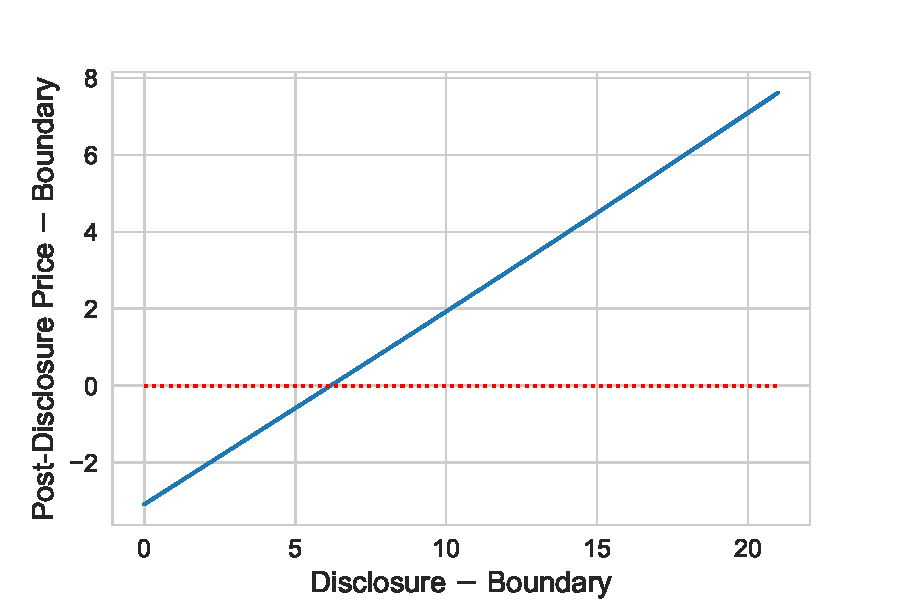
\includegraphics[scale=0.8]{Figures/DisclosurePostDisclosure.pdf}
\end{center}
\end{figure}

Figure \ref{fig2} shows that risk premia rise over time prior to disclosures.  The conditional distribution of the asset values is a mixture distribution, mixing over whether a firm already learned its value.  The probability of this event is initially small and rises over time, producing a rising covariance with the SDF.  It follows that announcement returns are higher on average when more time has passed prior to disclosure.

\begin{figure}[htp]\caption{The excess of the expected firm values over the price is shown as a function of time, assuming neither firm has yet disclosed.    The parameter values are $\mu=105$, $\mu^*=100$, and $\sigma=15$.\label{fig2}}
\begin{center}
    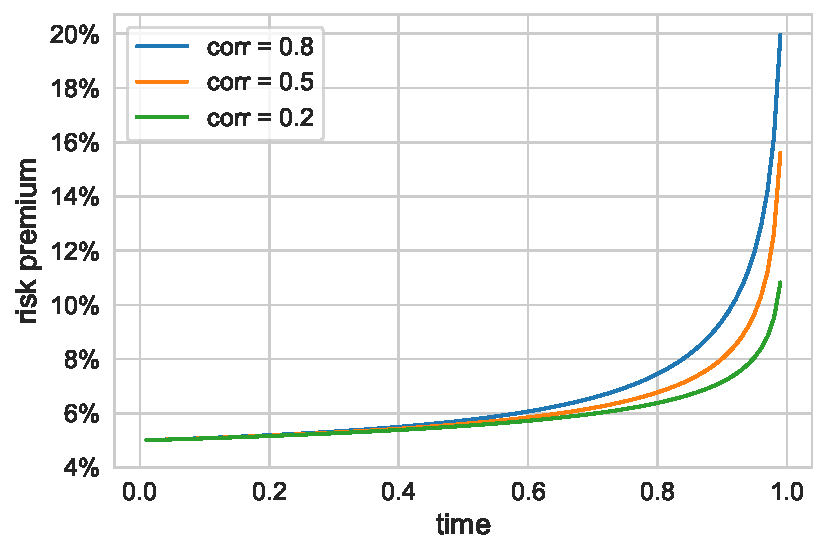
\includegraphics[scale=0.8]{Figures/RiskPremia.pdf}
\end{center}
\end{figure}

\section{Empirics}

We empirically examine information disclosure by firms in the context of earnings announcements. We test predictions from the model of the option value to delaying disclosure. We find that 75\% of firms irregularly make earnings announcements. We document evidence of strategic delay in information disclosure across industries and within industry. Across industries, we show that for industries where the option to delay is more valuable, earnings announcement dates are more dispersed. Within industry, we document that firms exercise the option value to delay in response to peer earnings announcements. When peer earnings announcement returns are abnormally positive, firms delay their earnings announcement date. Consistent with our model, we find evidence that firms exercise the option value to delay when choosing their earnings announcement dates. 

\subsection{Research Design and Data}\label{ss:researchdesign}

A necessary, but insufficient, requirement for firms to be strategically scheduling their earnings announcements in response to private information is that the market cannot perfectly predict their earnings announcement date. 

\begin{hypothesis}\label{hyp:surprisingdates}
Firm earnings announcements are not predictable with publicly available information to markets. 
\end{hypothesis}
To empirically test this hypothesis, we use data from Wall Street Horizons on firm earnings announcement dates. The data spans from 2007 to 2020 and reports the realized firm earnings announcement dates, which we denote $EA^{i}_{T}$ for firm $i$ and announcement date $T$. We also have data on the market's expectation of the firm's earnings announcement date, which we denote $E_{t}[EA^{i}_{T}]$ for the expectation as of calendar date $t$.  

We construct two measures to capture the unpredictability of earnings announcement dates. First, as a naive benchmark, we use the change from the previous year calendar earnings announcement date ($EAD^{i}_{T}$): 
\begin{equation}
    EAD^{i}_{T} =EA^{i}_{T} - EA^{i}_{T-4}
\end{equation}
where $EA^{i}_{T}$ is the earnings announcement date for firm $i$ for fiscal quarter $T$. For each firm, we measure the standard deviation in the year-on-year changes in earnings announcement dates ($\sigma_{EAD,i}$). This naive benchmark assumes that the best forecast for the firm's earnings announcement date is the previous year's earnings announcement date. However, some firms tend to follow patterns to their disclosure dates. For example, Boeing Company always announces their earnings on the third or fourth Wednesday of months January, April, July, and October. \cite{noh2021calendar} documents many such patterns to a subset of firms that predictably disclose earnings announcements. 

To best capture all available information to the market about firm earnings announcement dates, we use forecasts by Wall Street Horizons. %description of WSH forecasts% 

We define $EAS^{i}_{T}$ to be the difference between the firm's realized earnings announcement date and the Wall Street Horizons forecast of the earnings announcement date: 
\begin{equation}
    EAS^{i}_{T} =EA^{i}_{T} - E_{t}[EA^{i}_{T}].
\end{equation}
For each earnings announcement, we use the expected date as of the beginning of the earnings cycle ($t$). This scheduling surprise measure captures unpredictable shifts in the timing of earnings announcements. This measure is economically relevant because managers convey information to analysts about their expected schedule to future earnings announcements. Similarly, for each firm, we measure the standard deviation to earnings announcement date surprise ($\sigma_{EAS,i}$).

Firms tend to schedule their earnings announcements in advance of the announcement date. The median scheduled earnings announcement is scheduled 15 days in advance and is rarely revised. At first blush, scheduling earnings announcements in advance seems at odds with strategic delay. By scheduling in advance of the earnings date, firms give up the option of last minute adjustments to their earnings dates. However, firms may still behave strategically in scheduling earnings dates. For example, \cite{dehaan2015market} shows that firms with poor earnings news tend to schedule announcements when markets are less attentive (such as on Friday afternoon). Scheduling earnings announcements in advance increases the difficulty of strategically timing their earnings announcement compared to that of peer firms. Scheduling is an economic force that biases against us finding evidence of strategic timing of earnings disclosure. 


% A formal proposition or comparative statics in the model of this fact would be helpful to confirm whether this is a prediction of the model.
% Here are a few version of the proposition/comparative static that would be helpful in connecting with the empirics: 
1. The value of the option to delay increases in the dispersion of firm values ($\sigma_\varepsilon$). 
2. The dispersion in earnings announcement dates is increasing in the dispersion of firm values ($\sigma_\varepsilon$).  
3. Conditional on disclosure of the first firm, the expected delay in disclosure by the second firm is increasing in the dispersion of firm values ($\sigma_\varepsilon$).

The extent to which firm disclosure policies are influenced by the disclosures of peer firms depends on the correlation of firm values ($\rho$). We proxy for firm peer groups by industry and use three definitions of industry that are standard to the literature: Fama-French 12 industry portfolios \citep{fama1997industry}, 4-digit GICS grouping, and by TNIC \citep{hoberg2010product,hoberg2016text}.

Our first analysis uses cross-industry variation to identify the relationship between strategic delay and dispersion in firm values. To measure strategic delay, we use the dispersion in earnings announcement dates within an industry and earnings cycle. For industries where firms tend to strategically delay their disclosures, we expect that earnings announcement dates are more dispersed. To measure the dispersion in firm values, we use the dispersion in abnormal earnings announcement returns within an industry. The identifying assumption is that dispersion in firm values is positively associated with more surprising announcement returns. 

We empirically test the hypothesis that industries for which firms have more dispersed earnings news also feature more strategic delay. 
\begin{hypothesis}\label{hyp:crossindustry}
Firms within industries that have more dispersed earnings announcement returns also have more dispersed earnings announcement dates. 
\end{hypothesis}

A positive correlation of cross-industry variation in dispersion of earnings announcement returns and earnings dates is suggestive, but not causal, evidence of strategic delay. To mitigate concerns about contemporaneous relationships with omitted variables, we use one earning cycle lagged dispersion in earnings announcement returns. On average a 1 percent increase in lagged industry dispersion in earnings announcement returns is associated with a 0.62 percent increase in current period dispersion. Despite using lagged dispersion in earnings announcement returns, there are many persistent unobservable industry characteristics that may generate a spurious relationship between dispersion in earnings announcement returns and dates. For example, variation in industry misclassification may cause a spurious relationship. Firms misclassified in an industry are likely to have both different earnings news and a different earnings cycle from the other firms within the industry. Therefore, industries with more misclassified firms may have both more dispersed earnings announcement returns and earnings dates. 

In addition to cross-industry variation, we use within-industry variation to test the core economic mechanism of the model: strategic delay in response to peer disclosures. For our peer disclosure information event, we use earnings announcements of firms within the same industry. The model predicts that firms delay their disclosures when peer firms disclose positive news and move forward their disclosures when peer firms disclose negative news. By using within-industry variation and peer earnings announcement news, we can saturate the hypothesis test with firm and time fixed effects. 

\begin{hypothesis}\label{hyp:withinindustry}
Conditional on a positive (negative) disclosure by a peer firm, firms delay (move forward) their own disclosures.
\end{hypothesis}

The relevant timing of these peer firm earnings announcement returns are important to the economic mechanism. Consider the three announcements cases: expected $T_{X}$, early $T_{E}$, and delay $T_{D}$. Figure \ref{fig:Peer_Firm_Timing} illustrates these three cases and the relevant timing of peer firm earnings announcement returns. For the case where the firm announces its earnings when the market expected ($T_{X}$), then the firm chose to announce after the market observed peer earnings announcement returns in the days prior to $T_{X}$. For the case where the firm announces early, there is a different set of relevant peer announcements. The model predicts that the firm chose to announce early due to positive peer firm earnings announcement returns leading up to $T_{E}$. For the case where the firm delays its earnings announcement, the model predicts that the firm made this decision because of positive peer earnings announcement returns prior to its expected announcement date ($T_{E}$). When the firm made the decision to delay, the market has yet to observe the peer earnings announcement returns leading up to $T_{D}$. Therefore, we define the relevant timing of peer firm excess earnings announcement returns as a 3-day window by case:

\begin{equation}
      \tau=
    \begin{cases}
      \{T_{E}-3,T_{E}-2,T_{E}-1\} & \text{if early disclosure}\\
      \{T_{X}-3,T_{X}-2,T_{X}-1\} & \text{if expected or delayed disclosure}
    \end{cases}     
\end{equation}

To measure excess earnings announcement returns for the aggregate market, we use data from CRSP to measure excess returns to the 3-factor Fama-French model for each earnings announcement date of firm $i$:  
\begin{equation}
    ER^{Agg}_{t}= \sum_{i, \tau} w_{i} ER^{i}
\end{equation}
where the weight $w_i$ is the ratio of firm $i$ market capitalization to the sum of the market capitalization of all announcing firms within the relevant time window $\tau$. Similarly, we estimate peer excess earnings announcement returns by subsampling to the firms within the same industry: 
\begin{equation}
    ER^{Ind}_{t}= \sum_{i\in Ind,\tau} w_{i} ER^{i}
\end{equation}
where we restrict the sum to all firms within industry $Ind$. 

To focus on firms that respond to peer news, we sub-sample to the firms that report earnings in the latter half of the earnings cycle. We empirically test whether these firms strategically respond to peer firms that announced earlier in the earnings cycle. We estimate by OLS
\begin{equation} \label{eq:withinindustry}
    EAS^{i}_{t} = \alpha_{i} +\alpha_{t} + \beta ER^{Agg}_{\tau} + \gamma  ER^{Ind(i)}_{\tau}  + \epsilon_{i,t}
\end{equation}
where $\alpha_{i}$ is a firm fixed effect, $\alpha_{t}$ is a time fixed effect for the earnings announcement date, $ER^{Agg}_{\tau}$ and $ER^{Ind(i)}_{\tau}$ are the weighted average of earnings announcement excess returns of all other firms and industry peers for the relevant time window $\tau$. 

If firms strategically delay in response to positive peer news and move forward in response to negative peer news (\ref{hyp:withinindustry}), we expect to find positive $\beta$ (all potential peers) and $\gamma$ (industry-specific peers). 


\subsection{Empirical Results}\label{ss:empiricalresults}

In this subsection, we present and discuss the empirical findings in relation to the hypotheses described in \ref{ss:researchdesign}. 

Following the literature, we restrict the sample to firms with a share price greater than \$5 and a market capitalization greater than 50 million. Furthermore, we require that Wall Street Horizons covers the firm in forecasting its earnings announcement date. From the earnings announcement literature, we also require that the firm have a standard fiscal cycle with quarter-ends that match calendar quarter-ends.\footnote{This subsamples firms to those which have regular earnings cycles for fiscal quarter-ends of March 31st, June 30th, September 31st, and December 31st.} We have data on 5,816 firms and 149,059 firm-quarter observations.

At the beginning of an earnings cycle, earnings announcement date forecasts have an average absolute error of 3.1 days and a standard deviation of 4.5 days. Forecast error is the difference between the realized and forecasted earnings announcement date ($EAS^{i}_{T}$). However, forecast errors vary across firms, where the bottom 10th percentile of firms have an average absolute forecast error of 1.5 days, while the top 90th percentile have an average absolute forecast error of 7.1 days. 

The forecast errors by professional forecasters of earnings announcements correlate with realized year-on-year calendar changes in earnings announcement dates. The forecast errors ($EAS^{i}_{T}$) and calendar day changes ($EAD^{i}_{T}$) have a correlation of 77\%. Figure \ref{fig:EA_Shifts} plots the distribution of $EAS^{i}_{T}$ and $EAD^{i}_{T}$. Although the measures are winsorized at the 1\% level, there are outlier forecast errors and calendar changes in excess of 10 days. 

Following \cite{noh2021calendar}, we look for calendar date patterns to earnings announcement dates. On average firms, announce 60\% of their earnings announcements on the same day of the week for each earnings cycle. This firm-level propensity to announce on the same day of the week is significantly higher than by chance. Across all firms, the most popular announcement day of the week is Thursday, on which 33\% of earnings announcements are made. Firms with unpredictable earnings announcement dates are less likely to announce on the same day of the week. Firms in the 90th percentile of absolute earnings date forecast errors ($|EAS^{i}_{T}|$) are 11.4 percentage points less likely to announce on the same day of the week compared to firms in the 10th percentile. 

We find evidence that professional forecasters cannot perfectly predict earnings announcement dates. This unpredictability is supportive evidence of Hypothesis 1 and a necessary condition for firms to be strategically changing earnings announcements in response to private firm-information. Of interest is that the unpredictability of firm earnings announcement dates varies significantly in the cross-section of firms. 

This cross-sectional variation implies that some firms exercise their option to strategically delay disclosure, while other firms do not. We provide suggestive evidence of a trade off between strategic delay in earnings announcements and a firm's information environment. Table \ref{tab:summary_stats_predictable_size_matched} shows that for a size-matched sample of firms, firms with unpredictable earnings dates tend to have significantly lower earnings and revenue response coefficients and worse analyst forecasts (larger earnings and revenue surprise and disagreement among analysts). This evidence suggests that there is a cost to the firm exercising the option value of varying its earnings announcement date. 

For our subsequent analyses, we focus on firms that tend to have unpredictable earnings announcements. We exclude firms for which there tends to be no surprise to the earnings announcement date. For these firms, Wall Street Horizons exactly forecasts the announcement date for more than half of the firm's earnings announcements. Furthermore, we exclude firms that announce on the same day of the week for more than 90 percent of their earnings announcements. We exclude 1,468 firms that predictably announce earnings, which leaves us with a sample of 4,348 firms and 113,861 firm-quarter observations. 

%%%%Industry level analysis
We find substantial variation in the dispersion to earnings announcement dates by industry and earnings cycle. Figure \ref{fig:Industry_Date_Dispersion} plots this dispersion. Industry is measured at the 6-digit GICs level and dispersion is measured as the standard deviation to earnings cycle calendar dates. The dispersion of earnings dates varies from 5 days at the 10th percentile to 15 days at the 90th percentile. Approximately half of the variation to earnings date dispersion cannot be explained by industry fixed effects and earnings cycle fixed effects.

At the industry-level, we find a strong positive relationship between lagged industry-level dispersion in announcement excess returns and current dispersion in announcement dates. For each decile of dispersion of returns, figure \ref{fig:Industry_Date_Ret} plots the average dispersion in announcement dates. Going from the 1st decile of earnings announcement excess return dispersion to the 10th decile, the dispersion in announcement dates increases by 2 days. This effect is economically large compared to the 9.3 day average industry-cycle dispersion in announcement dates. This evidence is consistent with hypothesis \ref{hyp:crossindustry}. 

%%%%Firm level analysis
To better identify strategic delay, we use firm-level variation in earnings announcement dates and peer-firm announcement returns. We test hypothesis \ref{hyp:withinindustry} by estimating equation \ref{eq:withinindustry}. Table \ref{tab:Shifts_Peer_Returns} shows that firms delay their earnings announcements in response to aggregate and industry-level earnings announcement returns. We standardized each of the explanatory variables such that one unit is 1 standard deviation.  Table \ref{tab:Shifts_Peer_Returns_a} shows that for a 1 standard deviation increase in aggregate excess earnings announcement returns, firms delay their earnings announcements by 0.3 to 0.59 days. 

Furthermore, firms delay their earnings announcement date in response to positive excess earnings announcement returns for peer firms. This peer-firm effect is robust to all three measures of industry (Fama-French in column 3, GICS in column 4, and TNIC in column 5). Column 3 of table \ref{tab:Shifts_Peer_Returns_a} shows that for a 1 standard deviation increase in Fama-French peer-firm earnings announcement excess returns, firms delay by 0.12 days. These findings are robust to controlling for firm and time fixed effects. Time fixed effects are for the day of actual announcement, not the expected announcement date. Therefore, the aggregate excess earnings announcement return is not absorbed by the time fixed effect. The aggregate excess earnings announcement return is measured over dates $\tau$ which varies by firm in addition to time. 

The results are robust to measuring delay using calendar shifts, rather than market expectations of the earnings announcement date (table \ref{tab:Shifts_Peer_Returns_b}). 

Using firm-level variation, we find effects that are smaller in economic magnitude than that of the industry-level effects. However, the firm-level findings are better identified because we control for potential omitted variables through firm and time fixed effects. However, these fixed-effects may absorb much of the relevant economic variation to the strategic decision of firms to delay earnings announcements. 

% Should we relegate these robustness tables to the appendix? 
As robustness checks, we consider the following alternatives. First, we expand the sample to include firms that announce in the first half of the earnings cycle. These firms are less likely to be responding to peer earnings announcements because of their position in the earnings cycle. An outcome of the strategic disclosure model is that early announcing firms are more likely to be firms that have learned that they have a high value. The disclosure of these firms are less likely to be influence by peer firm disclosures. Table \ref{Shifts_Peer_Returns_Full} shows that the findings are robust to expanding the sample to include the early announcing firms. The results are qualitatively similar: firms delay in response to positive peer news and move forward in response to negative peer news. The findings are robust, except for the GICS peer grouping where we find a positive, but insignificant coefficient on peer firm returns. 

Second, we evaluate the robustness of our findings to a subsample of firms that delay their earnings announcements. The primary economic mechanism of the model is the strategic delay of earnings announcements. We test whether our primary empirical findings are robust to focusing on variation in how much firms delay their earnings announcements in response to peer firm announcements. Table \ref{tab:Shifts_Peer_Returns_Delays} shows that the findings are robust to the subsample of firms that delay. The results are qualitatively similar. 


\newpage{}
\bibliographystyle{jf}
\bibliography{disclosure}{}


%%%%%%%%%%%%%%%%%%%%%%%%%%%%%%%%%%%%%%%%%%%%%%
% Figures
%%%%%%%%%%%%%%%%%%%%%%%%%%%%%%%%%%%%%%%%%%%%%%

\newpage{}
\newpage \clearpage

%%%%%%%%%%%%%%%%%%%%%%%%%%%%
% Distribution of Shifts to Earnings Announcements
%%%%%%%%%%%%%%%%%%%%%%%%%%%%

\begin{figure}[ht]
    \begin{center}
    \caption{Distribution of Shifts to Earnings Announcements} \label{fig:EA_Shifts}
    \begin{subfigure}[t]{0.8\textwidth}
        \caption{Surprise Change to EA Date}
        \centering
        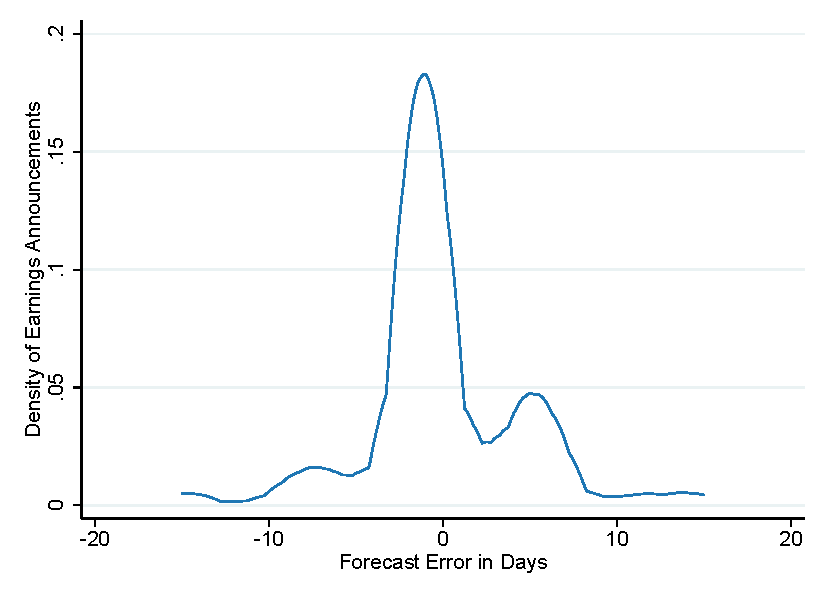
\includegraphics[width=\linewidth]{Figures/Date_Diff_w.pdf}  \label{fig:EA_Shifts_Surprise}
    \end{subfigure}
    \hfill
    \begin{subfigure}[t]{0.8\textwidth}
        \caption{Year-on-Year Change to EA Date}
    \centering
        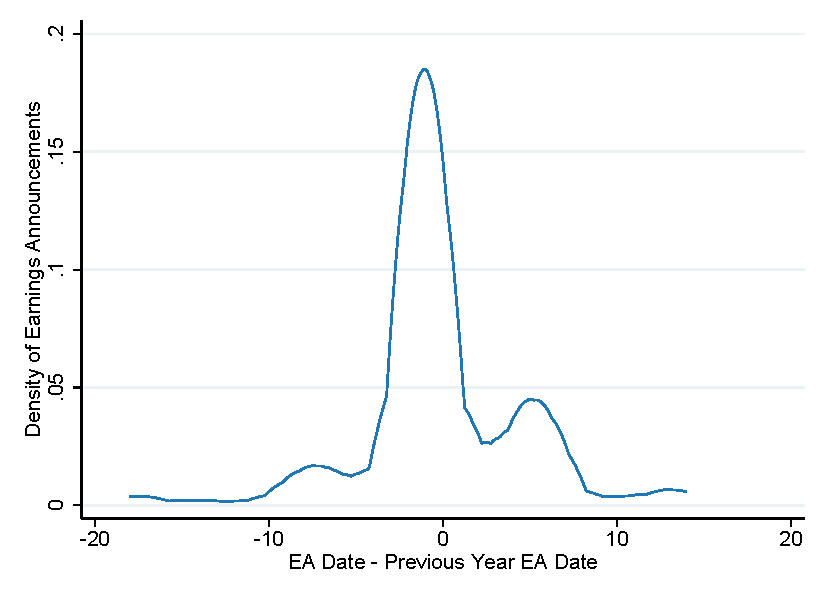
\includegraphics[width=\linewidth]{Figures/Doy_Diff.pdf}  \label{fig:EA_Shifts_YoY}
    \end{subfigure}
    \end{center}
\end{figure}




%%%%%%%%%%%%%%%%%%%%%%%%%%%%
% Industry level analysis 
%%%%%%%%%%%%%%%%%%%%%%%%%%%%
\begin{figure}[ht]
    \begin{center}
    \caption{Industry-Level Dispersion of EA Dates and Excess Returns} \label{fig:Industry}
    \begin{subfigure}[t]{0.8\textwidth}
        \caption{Industry-Level Dispersion of EA Dates}
        \centering
        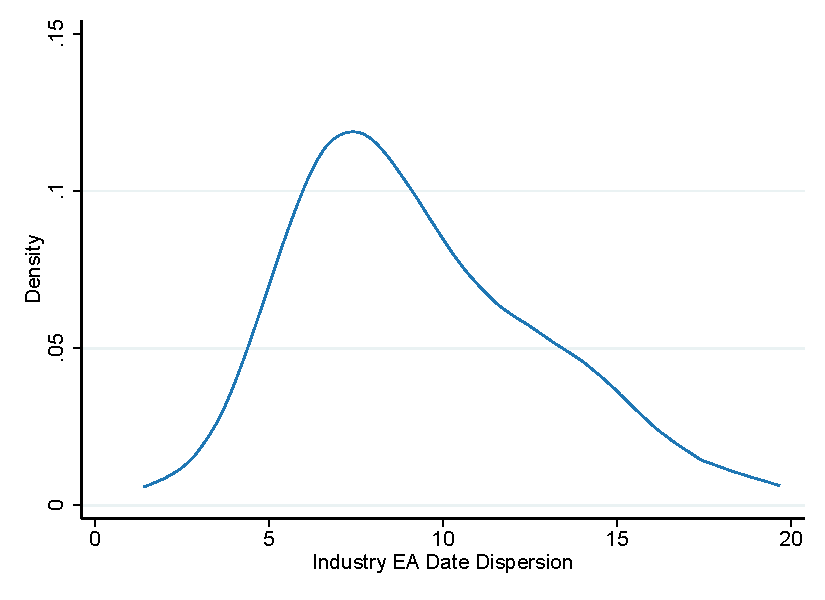
\includegraphics[width=\linewidth]{Figures/Industry EA Dispersion.pdf}  \label{fig:Industry_Date_Dispersion}
    \end{subfigure}
    \hfill
    \begin{subfigure}[t]{0.8\textwidth}
        \caption{Deciles of Industry EA Excess Return Dispersion and Date Dispersion}
    \centering
        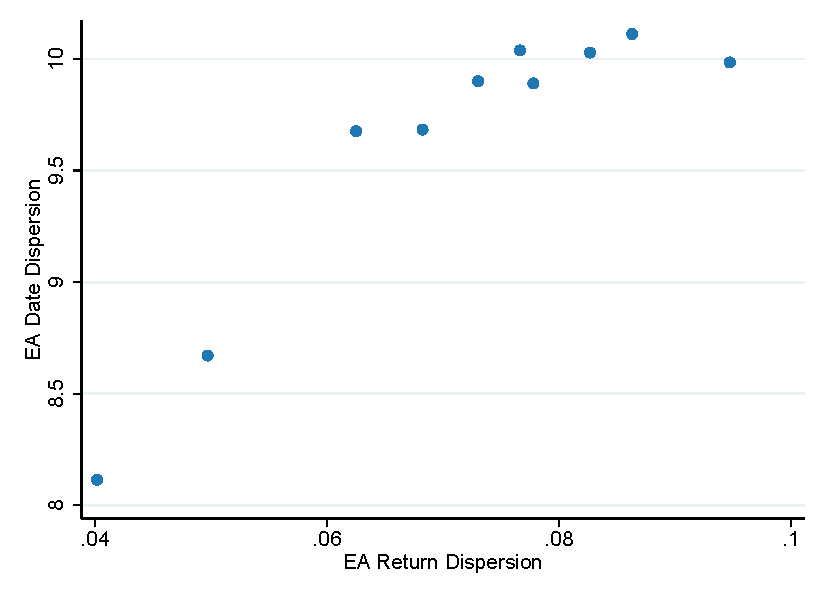
\includegraphics[width=\linewidth]{Figures/Industry EA Date and Return Dispersion.pdf}  \label{fig:Industry_Date_Ret}
    \end{subfigure}
    \end{center}
\end{figure}




%%%%%%%%%%%%%%%%%%%%%%%%%%%%
% Timing
%%%%%%%%%%%%%%%%%%%%%%%%%%%%
\begin{figure}[h]
    \caption{Relevant Time of Peer Firm Returns} \label{fig:Peer_Firm_Timing}
    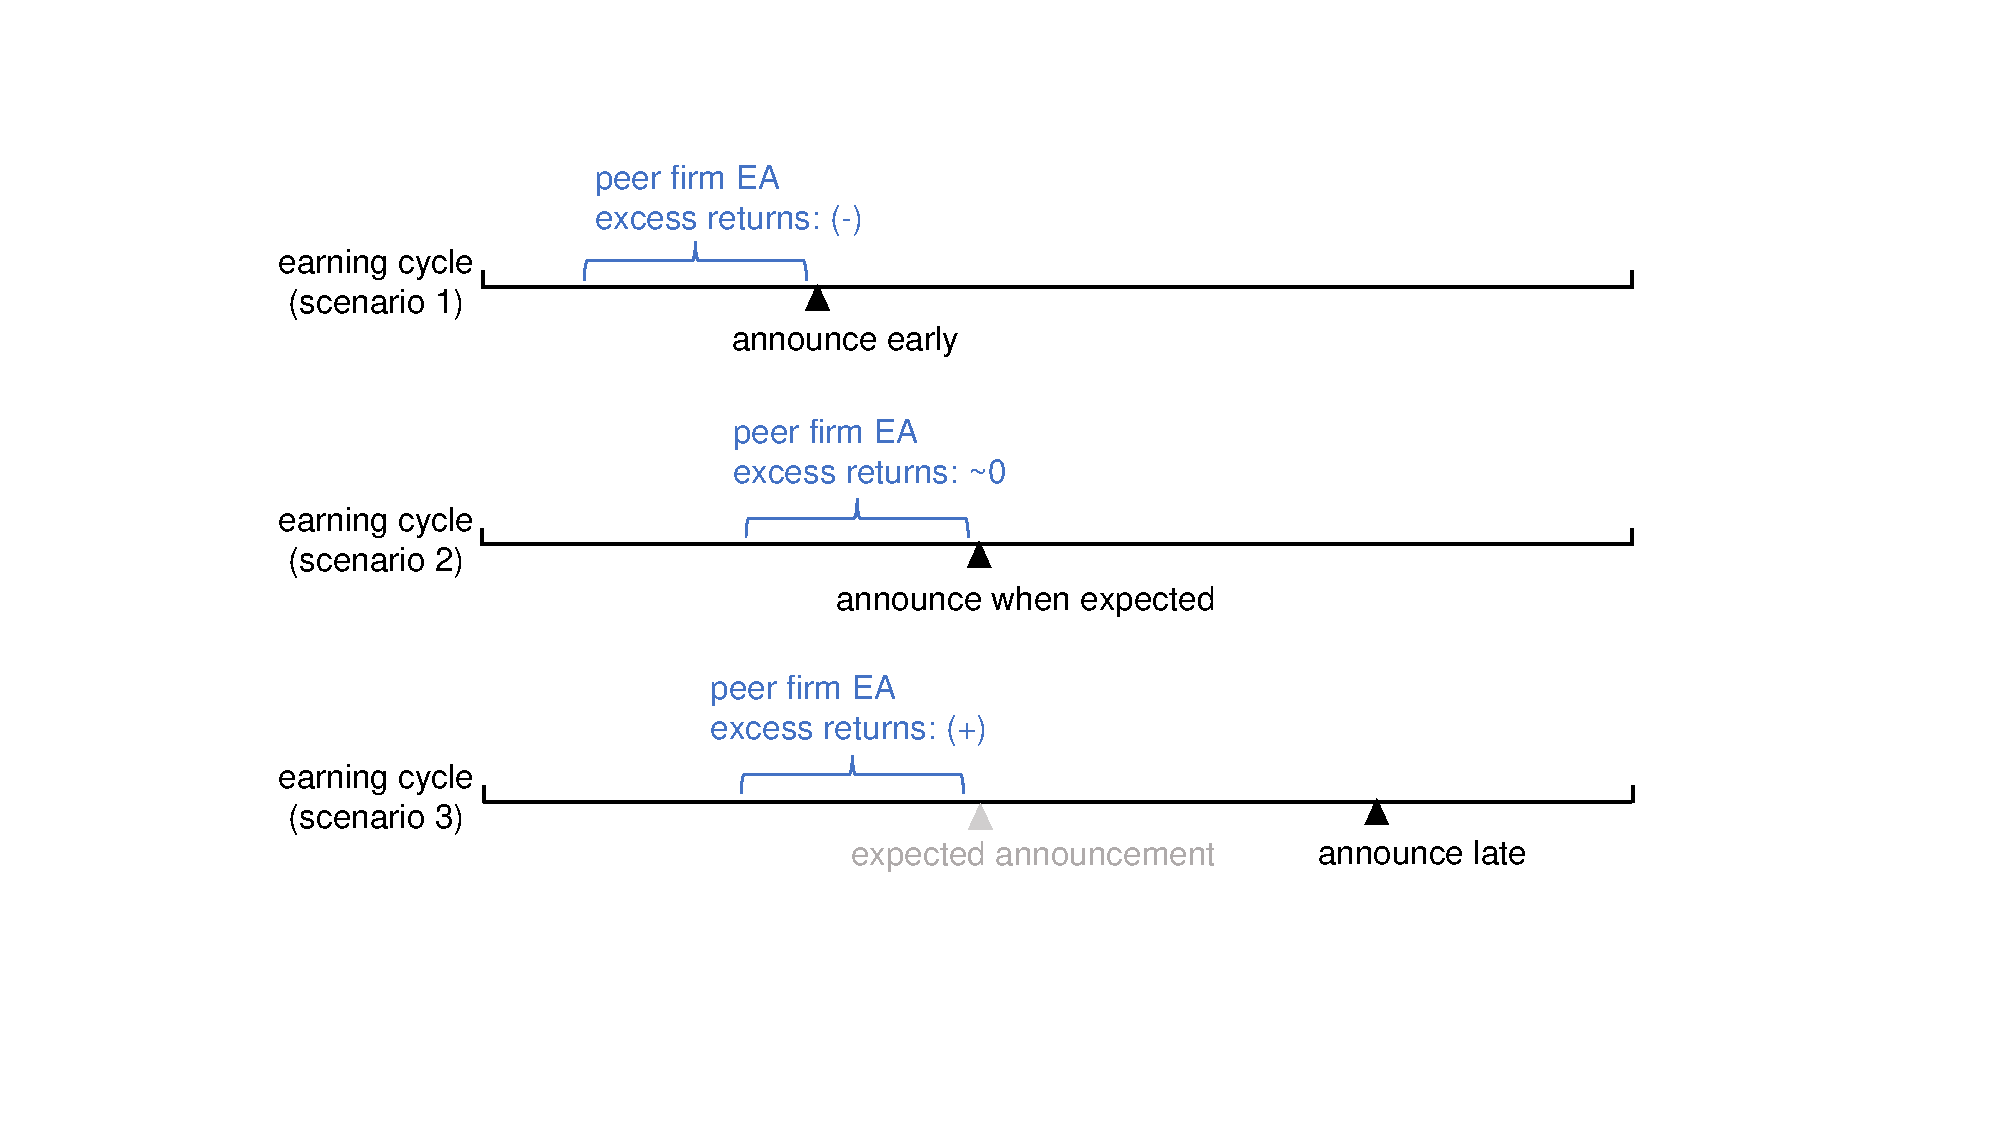
\includegraphics[width=\linewidth]{Figures/Hypothesis Graphs.pdf}  
\end{figure}

%%%%%%%%%%%%%%%%%%%%%%%%%%%%%%%%%%%%%%%%%%%%%%
% Tables
%%%%%%%%%%%%%%%%%%%%%%%%%%%%%%%%%%%%%%%%%%%%%%
\newpage{}
\newpage \clearpage

%%%%%%%%%%%%%%%%%%%%%%%%%%%%
% Summary statistics
%%%%%%%%%%%%%%%%%%%%%%%%%%%%
\begin{table}[h]
\caption{\label{tab:summary_stats} Summary Statistics}
\vspace{10pt}
\renewcommand{\arraystretch}{1.1}\makebox[\linewidth][c]{

{\small \input{Tables/Summary_stats}
}
} \vspace{10pt}

\emph{\footnotesize{}Notes}{\footnotesize{}: This table presents summary statistics for surprise shifts to forecasted earnings dates ($EAS_T^i$) and previous year earnings dates ($EAD_T^i$), excess earnings announcement returns for all firms ($ER^{Agg}_t$) and peer firms. We define peer firms by three industry groupings: Fama-French portfolios, GICS, and TNIC.}{\footnotesize\par}
\end{table}


%%%%%%%%%%%%%%%%%%%%%%%%%%%%
% Summary statistics size matched
%%%%%%%%%%%%%%%%%%%%%%%%%%%%
\newpage
\begin{table}[h]
\caption{\label{tab:summary_stats_predictable_size_matched} Sized Matched Summary Statistics for Firms with Predictable and Unpredictable Earnings Dates}
\vspace{10pt}
\renewcommand{\arraystretch}{0.8}\makebox[\linewidth][c]{

{\small \begin{tabular}{l*{8}{c}}
\toprule
            &           N&        Mean&          SD&        Diff&       TStat&          Q1&         Med&          Q2\\
\midrule
TA          &        1273&       7.613&       1.525&           &           &       6.641&       7.585&       8.588\\
          &        1273&       7.638&       1.538&       0.024&       0.403&       6.624&       7.586&       8.588\\
Equity / TA         &        1273&       0.586&       0.236&           &           &       0.415&       0.589&       0.767\\
         &        1273&       0.603&       0.250&       0.017&       1.729&       0.439&       0.605&       0.765\\
ROA         &        1273&       0.036&       0.076&           &           &       0.009&       0.033&       0.067\\
         &        1273&       0.022&       0.076&      -0.014&      -4.751&       0.006&       0.024&       0.053\\
Accrual SD    &        1273&       1.616&       1.663&           &           &       0.461&       1.206&       2.104\\
    &        1273&       1.706&       1.832&       0.089&       1.289&       0.504&       1.118&       2.235\\
Earnings Persistence        &        1273&       0.384&       0.344&           &           &       0.158&       0.402&       0.637\\
    &        1273&       0.371&       0.362&      -0.013&      -0.910&       0.131&       0.399&       0.618\\
ERC EPS      &        1168&      11.436&      18.938&           &           &       1.236&       5.618&      14.472\\
     &        1152&       8.397&      16.132&      -3.039&      -4.158&       0.961&       3.319&      10.256\\
ERC Revenue       &        1170&       0.439&       0.804&           &           &       0.025&       0.221&       0.662\\
      &        1156&       0.387&       0.786&      -0.052&      -1.570&       0.003&       0.184&       0.618\\
|Surprise EPS|&        1190&       0.496&       0.846&           &           &       0.122&       0.249&       0.518\\
&        1183&       0.779&       1.310&       0.283&       6.251&       0.164&       0.331&       0.769\\
|Surprise REV|&        1189&       5.927&       5.818&           &           &       2.432&       4.071&       7.068\\
&        1182&       7.160&       6.956&       1.233&       4.685&       2.666&       4.599&       8.906\\
Disagreement EPS&        1148&       0.276&       0.542&           &           &       0.067&       0.131&       0.266\\
&        1138&       0.456&       0.847&       0.180&       6.049&       0.096&       0.192&       0.394\\
Disagreement REV&        1139&       5.126&       6.487&           &           &       1.553&       2.718&       6.200\\
&        1125&       6.223&       7.675&       1.097&       3.676&       1.812&       3.297&       7.138\\
Analyst Coverage    &        1192&       1.747&       0.916&           &           &       1.344&       1.865&       2.347\\
     &        1189&       1.717&       0.900&      -0.029&      -0.784&       1.322&       1.842&       2.311\\
CAPM Beta       &        1273&       0.947&       0.299&           &           &       0.748&       0.952&       1.134\\
       &        1273&       0.982&       0.314&       0.035&       2.902&       0.781&       0.971&       1.189\\
\bottomrule
\end{tabular}

}
} \vspace{10pt}

\emph{\footnotesize{}Notes}{\footnotesize{}: This table presents summary statistics by whether the firm's earnings announcements are predictable. We group firms into above or below median predictability to earnings announcements. We sub-sample to a size-matched sample of firms. The first row for each variable is the group with above median predictability and the second row is for the group with below median predictability. Each observation is 1 firm. }{\footnotesize\par}
\end{table}




%%%%%%%%%%%%%%%%%%%%%%%%%%%%
% Shifts in EA 
%%%%%%%%%%%%%%%%%%%%%%%%%%%%
\begin{table}
\caption{Shifts in EA Dates in Response to Peer Firm EA Excess Returns}
\label{tab:Shifts_Peer_Returns}
\begin{subtable}{\linewidth}
\caption{Shift in Expected EA Date} \label{tab:Shifts_Peer_Returns_a}
\centering
\renewcommand{\arraystretch}{0.8}
\small{         {         \def\sym#1{\ifmmode^{#1}\else\(^{#1}\)\fi}         \begin{tabular}{l*{5}{c}}         \toprule          &\multicolumn{5}{c}{Dep Variable: Shift in Expectations} \\         \cmidrule(lr){2-6}           &\multicolumn{1}{c}{(1)}&\multicolumn{1}{c}{(2)} &\multicolumn{1}{c}{(3)}         &\multicolumn{1}{c}{(4)}        &\multicolumn{1}{c}{(5)} \\         
\midrule
Agg Ex Ret  &       0.295\sym{***}&       0.428\sym{***}&       0.402\sym{***}&       0.420\sym{***}&       0.589\sym{***}\\
            &      (0.08)         &      (0.12)         &      (0.12)         &      (0.12)         &      (0.15)         \\
FF Ex Ret   &                     &                     &       0.119\sym{***}&                     &                     \\
            &                     &                     &      (0.03)         &                     &                     \\
GICS Ex Ret &                     &                     &                     &       0.074\sym{**} &                     \\
            &                     &                     &                     &      (0.03)         &                     \\
TNIC Ex Ret &                     &                     &                     &                     &       0.094\sym{***}\\
            &                     &                     &                     &                     &      (0.03)         \\
         \cmidrule(lr){1-6}          \multicolumn{1}{l}{Firm FE} & Y&Y&Y&Y&Y \\         \multicolumn{1}{l}{Time FE} & N&Y&Y&Y&Y \\         
Adjusted $R^2$&        0.06         &        0.35         &        0.35         &        0.35         &        0.38         \\
$N$         &      61,804         &      61,392         &      61,392         &      61,387         &      51,322         \\
\bottomrule                         \end{tabular}                         }
}
\end{subtable}

\vspace{20pt}
\begin{subtable}{\linewidth}
\caption{Shift in Calendar EA Date} \label{tab:Shifts_Peer_Returns_b}
\centering
\renewcommand{\arraystretch}{0.8}
\small{         {         \def\sym#1{\ifmmode^{#1}\else\(^{#1}\)\fi}         \begin{tabular}{l*{5}{c}}         \toprule          &\multicolumn{5}{c}{Dep Variable: Shift in Calendar} \\         \cmidrule(lr){2-6}           &\multicolumn{1}{c}{(1)}&\multicolumn{1}{c}{(2)} &\multicolumn{1}{c}{(3)}         &\multicolumn{1}{c}{(4)}        &\multicolumn{1}{c}{(5)} \\         
\midrule
Agg Ex Ret  &       0.199\sym{***}&       0.310\sym{***}&       0.289\sym{***}&       0.304\sym{***}&       0.469\sym{***}\\
            &      (0.06)         &      (0.11)         &      (0.11)         &      (0.11)         &      (0.13)         \\
FF Ex Ret   &                     &                     &       0.094\sym{***}&                     &                     \\
            &                     &                     &      (0.03)         &                     &                     \\
GICS Ex Ret &                     &                     &                     &       0.042         &                     \\
            &                     &                     &                     &      (0.03)         &                     \\
TNIC Ex Ret &                     &                     &                     &                     &       0.071\sym{**} \\
            &                     &                     &                     &                     &      (0.03)         \\
         \cmidrule(lr){1-6}          \multicolumn{1}{l}{Firm FE} & Y&Y&Y&Y&Y \\         \multicolumn{1}{l}{Time FE} & N&Y&Y&Y&Y \\         
Adjusted $R^2$&        0.06         &        0.22         &        0.22         &        0.22         &        0.25         \\
$N$         &      54,059         &      53,680         &      53,680         &      53,675         &      45,661         \\
\bottomrule                         \end{tabular}                         }
}
\end{subtable}
\end{table}



%%%%%%%%%%%%%%%%%%%%%%%%%%%%
% Shifts in EA Full Sample
%%%%%%%%%%%%%%%%%%%%%%%%%%%%
\begin{table}
\caption{Shifts in EA Dates in Response to Peer Firm EA Excess Returns \\
Robustness to Including Early-Cycle Firms}
\label{tab:Shifts_Peer_Returns_Full}
\begin{subtable}{\linewidth}
\caption{Shift in Expected EA Date} \label{tab:Shifts_Peer_Returns_a}
\centering
\renewcommand{\arraystretch}{0.8}
\small{         {         \def\sym#1{\ifmmode^{#1}\else\(^{#1}\)\fi}         \begin{tabular}{l*{5}{c}}         \toprule          &\multicolumn{5}{c}{Dep Variable: Shift in Expectations} \\         \cmidrule(lr){2-6}           &\multicolumn{1}{c}{(1)}&\multicolumn{1}{c}{(2)} &\multicolumn{1}{c}{(3)}         &\multicolumn{1}{c}{(4)}        &\multicolumn{1}{c}{(5)} \\         
\midrule
Agg Ex Ret  &       0.146\sym{***}&       0.197\sym{**} &       0.185\sym{*}  &       0.197\sym{**} &       0.265\sym{**} \\
            &      (0.05)         &      (0.10)         &      (0.10)         &      (0.10)         &      (0.11)         \\
FF Ex Ret   &                     &                     &       0.053\sym{**} &                     &                     \\
            &                     &                     &      (0.02)         &                     &                     \\
GICS Ex Ret &                     &                     &                     &       0.005         &                     \\
            &                     &                     &                     &      (0.02)         &                     \\
TNIC Ex Ret &                     &                     &                     &                     &       0.086\sym{***}\\
            &                     &                     &                     &                     &      (0.02)         \\
         \cmidrule(lr){1-6}          \multicolumn{1}{l}{Firm FE} & Y&Y&Y&Y&Y \\         \multicolumn{1}{l}{Time FE} & N&Y&Y&Y&Y \\         
Adjusted $R^2$&        0.04         &        0.31         &        0.31         &        0.31         &        0.33         \\
$N$         &     113,861         &     113,413         &     113,397         &     113,401         &      96,778         \\
\bottomrule                         \end{tabular}                         }
}
\end{subtable}

\vspace{20pt}
\begin{subtable}{\linewidth}
\caption{Shift in Calendar EA Date} \label{tab:Shifts_Peer_Returns_b}
\centering
\renewcommand{\arraystretch}{0.8}
\small{         {         \def\sym#1{\ifmmode^{#1}\else\(^{#1}\)\fi}         \begin{tabular}{l*{5}{c}}         \toprule          &\multicolumn{5}{c}{Dep Variable: Shift in Calendar} \\         \cmidrule(lr){2-6}           &\multicolumn{1}{c}{(1)}&\multicolumn{1}{c}{(2)} &\multicolumn{1}{c}{(3)}         &\multicolumn{1}{c}{(4)}        &\multicolumn{1}{c}{(5)} \\         
\midrule
Agg Ex Ret  &       0.108\sym{**} &       0.159\sym{*}  &       0.145\sym{*}  &       0.158\sym{*}  &       0.238\sym{**} \\
            &      (0.05)         &      (0.09)         &      (0.08)         &      (0.09)         &      (0.09)         \\
FF Ex Ret   &                     &                     &       0.060\sym{***}&                     &                     \\
            &                     &                     &      (0.02)         &                     &                     \\
GICS Ex Ret &                     &                     &                     &       0.012         &                     \\
            &                     &                     &                     &      (0.02)         &                     \\
TNIC Ex Ret &                     &                     &                     &                     &       0.071\sym{***}\\
            &                     &                     &                     &                     &      (0.02)         \\
         \cmidrule(lr){1-6}          \multicolumn{1}{l}{Firm FE} & Y&Y&Y&Y&Y \\         \multicolumn{1}{l}{Time FE} & N&Y&Y&Y&Y \\         
Adjusted $R^2$&        0.02         &        0.20         &        0.20         &        0.20         &        0.22         \\
$N$         &     102,143         &     101,703         &     101,687         &     101,691         &      87,849         \\
\bottomrule                         \end{tabular}                         }
}
\end{subtable}
\end{table}



%%%%%%%%%%%%%%%%%%%%%%%%%%%%
% Delays only 
%%%%%%%%%%%%%%%%%%%%%%%%%%%%
\begin{table}
\label{tab:Shifts_Peer_Returns_Delays}
\caption{Shifts in EA Dates in Response to Peer Firm EA Excess Returns \\
Robustness to the Subsample of Firms that Delay}
\begin{subtable}{\linewidth}
\caption{Shift in Expected EA Date} \label{tab:Shifts_Peer_Returns_Delays_a}
\centering
\renewcommand{\arraystretch}{0.8}
\small{         {         \def\sym#1{\ifmmode^{#1}\else\(^{#1}\)\fi}         \begin{tabular}{l*{5}{c}}         \toprule          &\multicolumn{5}{c}{Dep Variable: Shift in Expectations} \\         \cmidrule(lr){2-6}           &\multicolumn{1}{c}{(1)}&\multicolumn{1}{c}{(2)} &\multicolumn{1}{c}{(3)}         &\multicolumn{1}{c}{(4)}        &\multicolumn{1}{c}{(5)} \\         
\midrule
Agg Ex Ret  &       0.216\sym{***}&       0.294\sym{***}&       0.265\sym{***}&       0.286\sym{***}&       0.423\sym{***}\\
            &      (0.08)         &      (0.10)         &      (0.10)         &      (0.10)         &      (0.12)         \\
FF Ex Ret   &                     &                     &       0.131\sym{***}&                     &                     \\
            &                     &                     &      (0.03)         &                     &                     \\
GICS Ex Ret &                     &                     &                     &       0.072\sym{**} &                     \\
            &                     &                     &                     &      (0.03)         &                     \\
TNIC Ex Ret &                     &                     &                     &                     &       0.104\sym{***}\\
            &                     &                     &                     &                     &      (0.03)         \\
         \cmidrule(lr){1-6}          \multicolumn{1}{l}{Firm FE} & Y&Y&Y&Y&Y \\         \multicolumn{1}{l}{Time FE} & N&Y&Y&Y&Y \\         
Adjusted $R^2$&        0.10         &        0.48         &        0.48         &        0.48         &        0.48         \\
$N$         &      44,713         &      44,268         &      44,268         &      44,263         &      38,366         \\
\bottomrule                         \end{tabular}                         }
}
\end{subtable}

\vspace{20pt}
\begin{subtable}{\linewidth}
\caption{Shift in Calendar EA Date} \label{tab:Shifts_Peer_Returns_Delays_b}
\centering
\renewcommand{\arraystretch}{0.8}
\small{         {         \def\sym#1{\ifmmode^{#1}\else\(^{#1}\)\fi}         \begin{tabular}{l*{5}{c}}         \toprule          &\multicolumn{5}{c}{Dep Variable: Shift in Calendar} \\         \cmidrule(lr){2-6}           &\multicolumn{1}{c}{(1)}&\multicolumn{1}{c}{(2)} &\multicolumn{1}{c}{(3)}         &\multicolumn{1}{c}{(4)}        &\multicolumn{1}{c}{(5)} \\         
\midrule
Agg Ex Ret  &       0.109\sym{*}  &       0.175\sym{*}  &       0.149\sym{*}  &       0.167\sym{*}  &       0.293\sym{***}\\
            &      (0.06)         &      (0.09)         &      (0.09)         &      (0.09)         &      (0.11)         \\
FF Ex Ret   &                     &                     &       0.117\sym{***}&                     &                     \\
            &                     &                     &      (0.03)         &                     &                     \\
GICS Ex Ret &                     &                     &                     &       0.065\sym{**} &                     \\
            &                     &                     &                     &      (0.03)         &                     \\
TNIC Ex Ret &                     &                     &                     &                     &       0.072\sym{**} \\
            &                     &                     &                     &                     &      (0.03)         \\
         \cmidrule(lr){1-6}          \multicolumn{1}{l}{Firm FE} & Y&Y&Y&Y&Y \\         \multicolumn{1}{l}{Time FE} & N&Y&Y&Y&Y \\         
Adjusted $R^2$&        0.11         &        0.31         &        0.31         &        0.31         &        0.31         \\
$N$         &      39,231         &      38,812         &      38,812         &      38,807         &      33,865         \\
\bottomrule                         \end{tabular}                         }
}
\end{subtable}
\end{table}











\end{document}

